\documentclass[twoside]{book}

% Packages required by doxygen
\usepackage{fixltx2e}
\usepackage{calc}
\usepackage{doxygen}
\usepackage[export]{adjustbox} % also loads graphicx
\usepackage{graphicx}
\usepackage[utf8]{inputenc}
\usepackage{makeidx}
\usepackage{multicol}
\usepackage{multirow}
\PassOptionsToPackage{warn}{textcomp}
\usepackage{textcomp}
\usepackage[nointegrals]{wasysym}
\usepackage[table]{xcolor}

% Font selection
\usepackage[T1]{fontenc}
\usepackage[scaled=.90]{helvet}
\usepackage{courier}
\usepackage{amssymb}
\usepackage{sectsty}
\renewcommand{\familydefault}{\sfdefault}
\allsectionsfont{%
  \fontseries{bc}\selectfont%
  \color{darkgray}%
}
\renewcommand{\DoxyLabelFont}{%
  \fontseries{bc}\selectfont%
  \color{darkgray}%
}
\newcommand{\+}{\discretionary{\mbox{\scriptsize$\hookleftarrow$}}{}{}}

% Page & text layout
\usepackage{geometry}
\geometry{%
  a4paper,%
  top=2.5cm,%
  bottom=2.5cm,%
  left=2.5cm,%
  right=2.5cm%
}
\tolerance=750
\hfuzz=15pt
\hbadness=750
\setlength{\emergencystretch}{15pt}
\setlength{\parindent}{0cm}
\setlength{\parskip}{3ex plus 2ex minus 2ex}
\makeatletter
\renewcommand{\paragraph}{%
  \@startsection{paragraph}{4}{0ex}{-1.0ex}{1.0ex}{%
    \normalfont\normalsize\bfseries\SS@parafont%
  }%
}
\renewcommand{\subparagraph}{%
  \@startsection{subparagraph}{5}{0ex}{-1.0ex}{1.0ex}{%
    \normalfont\normalsize\bfseries\SS@subparafont%
  }%
}
\makeatother

% Headers & footers
\usepackage{fancyhdr}
\pagestyle{fancyplain}
\fancyhead[LE]{\fancyplain{}{\bfseries\thepage}}
\fancyhead[CE]{\fancyplain{}{}}
\fancyhead[RE]{\fancyplain{}{\bfseries\leftmark}}
\fancyhead[LO]{\fancyplain{}{\bfseries\rightmark}}
\fancyhead[CO]{\fancyplain{}{}}
\fancyhead[RO]{\fancyplain{}{\bfseries\thepage}}
\fancyfoot[LE]{\fancyplain{}{}}
\fancyfoot[CE]{\fancyplain{}{}}
\fancyfoot[RE]{\fancyplain{}{\bfseries\scriptsize Generated by Doxygen }}
\fancyfoot[LO]{\fancyplain{}{\bfseries\scriptsize Generated by Doxygen }}
\fancyfoot[CO]{\fancyplain{}{}}
\fancyfoot[RO]{\fancyplain{}{}}
\renewcommand{\footrulewidth}{0.4pt}
\renewcommand{\chaptermark}[1]{%
  \markboth{#1}{}%
}
\renewcommand{\sectionmark}[1]{%
  \markright{\thesection\ #1}%
}

% Indices & bibliography
\usepackage{natbib}
\usepackage[titles]{tocloft}
\setcounter{tocdepth}{3}
\setcounter{secnumdepth}{5}
\makeindex

% Hyperlinks (required, but should be loaded last)
\usepackage{ifpdf}
\ifpdf
  \usepackage[pdftex,pagebackref=true]{hyperref}
\else
  \usepackage[ps2pdf,pagebackref=true]{hyperref}
\fi
\hypersetup{%
  colorlinks=true,%
  linkcolor=blue,%
  citecolor=blue,%
  unicode%
}

% Custom commands
\newcommand{\clearemptydoublepage}{%
  \newpage{\pagestyle{empty}\cleardoublepage}%
}

\usepackage{caption}
\captionsetup{labelsep=space,justification=centering,font={bf},singlelinecheck=off,skip=4pt,position=top}

%===== C O N T E N T S =====

\begin{document}

% Titlepage & ToC
\hypersetup{pageanchor=false,
             bookmarksnumbered=true,
             pdfencoding=unicode
            }
\pagenumbering{alph}
\begin{titlepage}
\vspace*{7cm}
\begin{center}%
{\Large Assignment 3 }\\
\vspace*{1cm}
{\large Generated by Doxygen 1.8.13}\\
\end{center}
\end{titlepage}
\clearemptydoublepage
\pagenumbering{roman}
\tableofcontents
\clearemptydoublepage
\pagenumbering{arabic}
\hypersetup{pageanchor=true}

%--- Begin generated contents ---
\chapter{Namespace Index}
\section{Packages}
Here are the packages with brief descriptions (if available)\+:\begin{DoxyCompactList}
\item\contentsline{section}{\hyperlink{namespacesrc}{src} }{\pageref{namespacesrc}}{}
\end{DoxyCompactList}

\chapter{Hierarchical Index}
\section{Class Hierarchy}
This inheritance list is sorted roughly, but not completely, alphabetically\+:\begin{DoxyCompactList}
\item \contentsline{section}{src.\+AttributeT}{\pageref{classsrc_1_1AttributeT}}{}
\item \contentsline{section}{src.\+CourseT}{\pageref{classsrc_1_1CourseT}}{}
\item \contentsline{section}{src.\+IndicatorT}{\pageref{enumsrc_1_1IndicatorT}}{}
\item \contentsline{section}{src.\+L\+OsT}{\pageref{classsrc_1_1LOsT}}{}
\item \contentsline{section}{src.\+Norm}{\pageref{classsrc_1_1Norm}}{}
\item \contentsline{section}{src.\+Services}{\pageref{classsrc_1_1Services}}{}
\item Hash\+Set\begin{DoxyCompactList}
\item \contentsline{section}{src.\+ProgramT}{\pageref{classsrc_1_1ProgramT}}{}
\end{DoxyCompactList}
\end{DoxyCompactList}

\chapter{Class Index}
\section{Class List}
Here are the classes, structs, unions and interfaces with brief descriptions\+:\begin{DoxyCompactList}
\item\contentsline{section}{\hyperlink{classsrc_1_1AttributeT}{src.\+AttributeT} }{\pageref{classsrc_1_1AttributeT}}{}
\item\contentsline{section}{\hyperlink{classsrc_1_1CourseT}{src.\+CourseT} \\*Class for initializing and operating on \hyperlink{classsrc_1_1CourseT}{CourseT} objects }{\pageref{classsrc_1_1CourseT}}{}
\item\contentsline{section}{\hyperlink{enumsrc_1_1IndicatorT}{src.\+IndicatorT} }{\pageref{enumsrc_1_1IndicatorT}}{}
\item\contentsline{section}{\hyperlink{classsrc_1_1LOsT}{src.\+L\+OsT} }{\pageref{classsrc_1_1LOsT}}{}
\item\contentsline{section}{\hyperlink{classsrc_1_1Norm}{src.\+Norm} }{\pageref{classsrc_1_1Norm}}{}
\item\contentsline{section}{\hyperlink{classsrc_1_1ProgramT}{src.\+ProgramT} }{\pageref{classsrc_1_1ProgramT}}{}
\item\contentsline{section}{\hyperlink{classsrc_1_1Services}{src.\+Services} }{\pageref{classsrc_1_1Services}}{}
\end{DoxyCompactList}

\chapter{File Index}
\section{File List}
Here is a list of all documented files with brief descriptions\+:\begin{DoxyCompactList}
\item\contentsline{section}{src/\hyperlink{CourseT_8java}{Course\+T.\+java} \\*Contains the Abstract Data Type for creating and operating with CourseT objects }{\pageref{CourseT_8java}}{}
\end{DoxyCompactList}

\chapter{Namespace Documentation}
\hypertarget{namespacesrc}{}\section{Package src}
\label{namespacesrc}\index{src@{src}}
\subsection*{Classes}
\begin{DoxyCompactItemize}
\item 
class \hyperlink{classsrc_1_1AttributeT}{AttributeT}
\item 
class \hyperlink{classsrc_1_1CourseT}{CourseT}
\begin{DoxyCompactList}\small\item\em Class for initializing and operating on \hyperlink{classsrc_1_1CourseT}{CourseT} objects. \end{DoxyCompactList}\item 
enum \hyperlink{enumsrc_1_1IndicatorT}{IndicatorT}
\item 
class \hyperlink{classsrc_1_1LOsT}{L\+OsT}
\item 
interface {\bfseries Measures}
\item 
class \hyperlink{classsrc_1_1Norm}{Norm}
\item 
class \hyperlink{classsrc_1_1ProgramT}{ProgramT}
\item 
class \hyperlink{classsrc_1_1Services}{Services}
\end{DoxyCompactItemize}


\subsection{Detailed Description}
Author\+: Mohammad Omar Zahir -\/ zahirm1 Revised\+: March 29 2021

Description\+: File for the \hyperlink{enumsrc_1_1IndicatorT}{IndicatorT} enumerator

Author\+: Mohammad Omar Zahir Revised\+: 29 March, 2021

Description\+: Contains the Abstract Data Type for creating and operating with \hyperlink{classsrc_1_1AttributeT}{AttributeT} objects

Author\+: Mohammad Omar Zahir -\/ zahirm1 Revised\+: March 29 2021

Description\+: Contains the interface for Measures that will be implemented and overriden by other classes

Author\+: Mohammad Omar Zahir -\/ zahirm1 Revised\+: March 29 2021

Description\+: File for the services module that contains a functions to determine the normal

Author\+: Mohammad Omar Zahir Revised\+: 29 March, 2021

Description\+: File for the \hyperlink{classsrc_1_1Norm}{Norm} Abstract object that specifies various boolean properties for other methods

Author\+: Mohammad Omar Zahir -\/ zahirm1 Revised\+: March 29 2021

Description\+: Contains the Abstract Data Type for creating and operating with \hyperlink{classsrc_1_1LOsT}{L\+OsT} objects

Author\+: Mohammad Omar Zahir Revised\+: 29 March, 2021

Description\+: Contains the Abstract Data Type for creating and operating with \hyperlink{classsrc_1_1ProgramT}{ProgramT} objects on the object 
\chapter{Class Documentation}
\hypertarget{classsrc_1_1AttributeT}{}\section{src.\+AttributeT Class Reference}
\label{classsrc_1_1AttributeT}\index{src.\+AttributeT@{src.\+AttributeT}}
\subsection*{Public Member Functions}
\begin{DoxyCompactItemize}
\item 
\mbox{\Hypertarget{classsrc_1_1AttributeT_a137984486b1eb74903cf556d09556a7b}\label{classsrc_1_1AttributeT_a137984486b1eb74903cf556d09556a7b}} 
{\bfseries AttributeT} (String attrib\+Name, \hyperlink{enumsrc_1_1IndicatorT}{IndicatorT}\mbox{[}$\,$\mbox{]} indicators)
\item 
\mbox{\Hypertarget{classsrc_1_1AttributeT_a5fcbd48378d0c08f9630bb44c70f7bb6}\label{classsrc_1_1AttributeT_a5fcbd48378d0c08f9630bb44c70f7bb6}} 
String {\bfseries get\+Name} ()
\item 
\mbox{\Hypertarget{classsrc_1_1AttributeT_a9f206678c126242c6d351a2cd973dc5d}\label{classsrc_1_1AttributeT_a9f206678c126242c6d351a2cd973dc5d}} 
\hyperlink{enumsrc_1_1IndicatorT}{IndicatorT} \mbox{[}$\,$\mbox{]} {\bfseries get\+Indicators} ()
\end{DoxyCompactItemize}


The documentation for this class was generated from the following file\+:\begin{DoxyCompactItemize}
\item 
src/Attribute\+T.\+java\end{DoxyCompactItemize}

\hypertarget{classsrc_1_1CourseT}{}\section{src.\+CourseT Class Reference}
\label{classsrc_1_1CourseT}\index{src.\+CourseT@{src.\+CourseT}}


Class for initializing and operating on \hyperlink{classsrc_1_1CourseT}{CourseT} objects.  




Inheritance diagram for src.\+CourseT\+:
\nopagebreak
\begin{figure}[H]
\begin{center}
\leavevmode
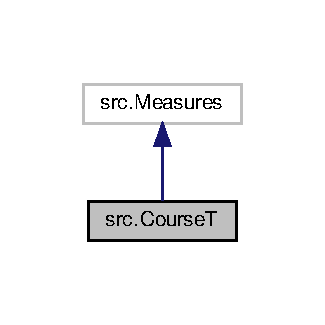
\includegraphics[width=156pt]{classsrc_1_1CourseT__inherit__graph}
\end{center}
\end{figure}


Collaboration diagram for src.\+CourseT\+:
\nopagebreak
\begin{figure}[H]
\begin{center}
\leavevmode
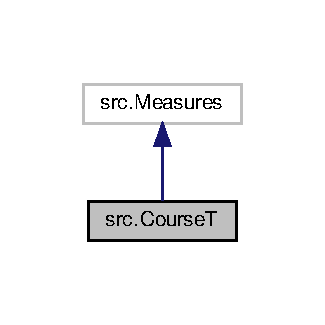
\includegraphics[width=156pt]{classsrc_1_1CourseT__coll__graph}
\end{center}
\end{figure}
\subsection*{Public Member Functions}
\begin{DoxyCompactItemize}
\item 
\hyperlink{classsrc_1_1CourseT_a1823da8802163805bfc9e387557730de}{CourseT} (String course\+Name, \hyperlink{enumsrc_1_1IndicatorT}{IndicatorT}\mbox{[}$\,$\mbox{]} indicators)
\begin{DoxyCompactList}\small\item\em Method for constructing the \hyperlink{classsrc_1_1CourseT}{CourseT} object. \end{DoxyCompactList}\item 
String \hyperlink{classsrc_1_1CourseT_a1cb1fbf76793e8b4f86946162acdb9a8}{get\+Name} ()
\begin{DoxyCompactList}\small\item\em Getter for returning the name of the \hyperlink{classsrc_1_1CourseT}{CourseT} object. \end{DoxyCompactList}\item 
\hyperlink{enumsrc_1_1IndicatorT}{IndicatorT} \mbox{[}$\,$\mbox{]} \hyperlink{classsrc_1_1CourseT_a303c3055b3a9ae2e80d0b7cfed58824f}{get\+Indicators} ()
\begin{DoxyCompactList}\small\item\em Getter for returning the array of \hyperlink{enumsrc_1_1IndicatorT}{IndicatorT} objects given at the time of initialization. \end{DoxyCompactList}\item 
\hyperlink{classsrc_1_1LOsT}{L\+OsT} \mbox{[}$\,$\mbox{]} \hyperlink{classsrc_1_1CourseT_aeec398eb1776b7b635a0f377b638992e}{get\+L\+Os} (\hyperlink{enumsrc_1_1IndicatorT}{IndicatorT} indicator)
\begin{DoxyCompactList}\small\item\em Method for retrieving the \hyperlink{classsrc_1_1LOsT}{L\+OsT} objects that are mapped to a given \hyperlink{enumsrc_1_1IndicatorT}{IndicatorT} object. \end{DoxyCompactList}\item 
void \hyperlink{classsrc_1_1CourseT_af1c3eb729e731d0b14f289655ce531ee}{add\+LO} (\hyperlink{enumsrc_1_1IndicatorT}{IndicatorT} indicator, \hyperlink{classsrc_1_1LOsT}{L\+OsT} outcome)
\begin{DoxyCompactList}\small\item\em Method for adding/mapping a given \hyperlink{classsrc_1_1LOsT}{L\+OsT} object to a given \hyperlink{enumsrc_1_1IndicatorT}{IndicatorT} object. \end{DoxyCompactList}\item 
void \hyperlink{classsrc_1_1CourseT_af325e1768e2368bb4588f13ac075cd2c}{del\+LO} (\hyperlink{enumsrc_1_1IndicatorT}{IndicatorT} indicator, \hyperlink{classsrc_1_1LOsT}{L\+OsT} outcome)
\begin{DoxyCompactList}\small\item\em Method for removing a given \hyperlink{classsrc_1_1LOsT}{L\+OsT} object that is mapped to a given \hyperlink{enumsrc_1_1IndicatorT}{IndicatorT} object. \end{DoxyCompactList}\item 
boolean \hyperlink{classsrc_1_1CourseT_a98d560017671e680b42c9d781eb9bb5a}{member} (\hyperlink{enumsrc_1_1IndicatorT}{IndicatorT} indicator, \hyperlink{classsrc_1_1LOsT}{L\+OsT}\mbox{[}$\,$\mbox{]} outcomes)
\begin{DoxyCompactList}\small\item\em Method for checking if a given \hyperlink{enumsrc_1_1IndicatorT}{IndicatorT} object exists with the given amount of \hyperlink{classsrc_1_1LOsT}{L\+OsT} objects mapped to it. \end{DoxyCompactList}\item 
double \mbox{[}$\,$\mbox{]} \hyperlink{classsrc_1_1CourseT_aa9abf592dff159aa10f74a7342296351}{measures} ()
\begin{DoxyCompactList}\small\item\em Implements the measure method from the Measure module that accepts no input. \end{DoxyCompactList}\item 
double \mbox{[}$\,$\mbox{]} \hyperlink{classsrc_1_1CourseT_ac81d229c59608e1848f077e9ac61d381}{measures} (\hyperlink{enumsrc_1_1IndicatorT}{IndicatorT} ind)
\begin{DoxyCompactList}\small\item\em Implements the measure method from the Measure module that accepts an \hyperlink{enumsrc_1_1IndicatorT}{IndicatorT} object. \end{DoxyCompactList}\item 
double \mbox{[}$\,$\mbox{]} \hyperlink{classsrc_1_1CourseT_a63d2487bf823e561f12fb06299b23ecd}{measures} (\hyperlink{classsrc_1_1AttributeT}{AttributeT} att)
\begin{DoxyCompactList}\small\item\em Implements the measure method from the Measure module that accepts an \hyperlink{enumsrc_1_1IndicatorT}{IndicatorT} object. \end{DoxyCompactList}\end{DoxyCompactItemize}


\subsection{Detailed Description}
Class for initializing and operating on \hyperlink{classsrc_1_1CourseT}{CourseT} objects. 

Consists of various functions, including the constructor, useful methods, getters, as well as the implementations of the measures methods from the Measures module. 

\subsection{Constructor \& Destructor Documentation}
\mbox{\Hypertarget{classsrc_1_1CourseT_a1823da8802163805bfc9e387557730de}\label{classsrc_1_1CourseT_a1823da8802163805bfc9e387557730de}} 
\index{src\+::\+CourseT@{src\+::\+CourseT}!CourseT@{CourseT}}
\index{CourseT@{CourseT}!src\+::\+CourseT@{src\+::\+CourseT}}
\subsubsection{\texorpdfstring{Course\+T()}{CourseT()}}
{\footnotesize\ttfamily src.\+Course\+T.\+CourseT (\begin{DoxyParamCaption}\item[{String}]{course\+Name,  }\item[{\hyperlink{enumsrc_1_1IndicatorT}{IndicatorT} \mbox{[}$\,$\mbox{]}}]{indicators }\end{DoxyParamCaption})}



Method for constructing the \hyperlink{classsrc_1_1CourseT}{CourseT} object. 


\begin{DoxyParams}{Parameters}
{\em course\+Name} & A String to represent the name. \\
\hline
{\em indicators} & An array of indicators to be stored in the course object.\\
\hline
\end{DoxyParams}
The constructor makes use of a Hashmap that maps an empty array of L\+Os objects to each of the indicators as separate keys. 

\subsection{Member Function Documentation}
\mbox{\Hypertarget{classsrc_1_1CourseT_af1c3eb729e731d0b14f289655ce531ee}\label{classsrc_1_1CourseT_af1c3eb729e731d0b14f289655ce531ee}} 
\index{src\+::\+CourseT@{src\+::\+CourseT}!add\+LO@{add\+LO}}
\index{add\+LO@{add\+LO}!src\+::\+CourseT@{src\+::\+CourseT}}
\subsubsection{\texorpdfstring{add\+L\+O()}{addLO()}}
{\footnotesize\ttfamily void src.\+Course\+T.\+add\+LO (\begin{DoxyParamCaption}\item[{\hyperlink{enumsrc_1_1IndicatorT}{IndicatorT}}]{indicator,  }\item[{\hyperlink{classsrc_1_1LOsT}{L\+OsT}}]{outcome }\end{DoxyParamCaption})}



Method for adding/mapping a given \hyperlink{classsrc_1_1LOsT}{L\+OsT} object to a given \hyperlink{enumsrc_1_1IndicatorT}{IndicatorT} object. 


\begin{DoxyParams}{Parameters}
{\em indicator} & An \hyperlink{enumsrc_1_1IndicatorT}{IndicatorT} object for mapping the L\+Os object to. \\
\hline
{\em outcome} & An \hyperlink{classsrc_1_1LOsT}{L\+OsT} object for mapping to the given \hyperlink{enumsrc_1_1IndicatorT}{IndicatorT} object.\\
\hline
\end{DoxyParams}
If the \hyperlink{enumsrc_1_1IndicatorT}{IndicatorT} object is found, the L\+Os object is only added if another L\+Os object of the same name does not exist there. If the \hyperlink{enumsrc_1_1IndicatorT}{IndicatorT} object does not exist, or the \hyperlink{classsrc_1_1LOsT}{L\+OsT} object already exists mapped to the \hyperlink{enumsrc_1_1IndicatorT}{IndicatorT} object, nothing is done. \mbox{\Hypertarget{classsrc_1_1CourseT_af325e1768e2368bb4588f13ac075cd2c}\label{classsrc_1_1CourseT_af325e1768e2368bb4588f13ac075cd2c}} 
\index{src\+::\+CourseT@{src\+::\+CourseT}!del\+LO@{del\+LO}}
\index{del\+LO@{del\+LO}!src\+::\+CourseT@{src\+::\+CourseT}}
\subsubsection{\texorpdfstring{del\+L\+O()}{delLO()}}
{\footnotesize\ttfamily void src.\+Course\+T.\+del\+LO (\begin{DoxyParamCaption}\item[{\hyperlink{enumsrc_1_1IndicatorT}{IndicatorT}}]{indicator,  }\item[{\hyperlink{classsrc_1_1LOsT}{L\+OsT}}]{outcome }\end{DoxyParamCaption})}



Method for removing a given \hyperlink{classsrc_1_1LOsT}{L\+OsT} object that is mapped to a given \hyperlink{enumsrc_1_1IndicatorT}{IndicatorT} object. 


\begin{DoxyParams}{Parameters}
{\em indicator} & An \hyperlink{enumsrc_1_1IndicatorT}{IndicatorT} object that has the L\+Os object mapped to it. \\
\hline
{\em outcome} & An \hyperlink{classsrc_1_1LOsT}{L\+OsT} object that is mapped to the given \hyperlink{enumsrc_1_1IndicatorT}{IndicatorT} object.\\
\hline
\end{DoxyParams}
If the \hyperlink{enumsrc_1_1IndicatorT}{IndicatorT} object is found, the L\+Os object is only removed if an L\+Os object of the same name exists there. If the \hyperlink{enumsrc_1_1IndicatorT}{IndicatorT} object does not exist, or the \hyperlink{classsrc_1_1LOsT}{L\+OsT} object of the same name does not exist mapped to the \hyperlink{enumsrc_1_1IndicatorT}{IndicatorT} object, nothing is done. \mbox{\Hypertarget{classsrc_1_1CourseT_a303c3055b3a9ae2e80d0b7cfed58824f}\label{classsrc_1_1CourseT_a303c3055b3a9ae2e80d0b7cfed58824f}} 
\index{src\+::\+CourseT@{src\+::\+CourseT}!get\+Indicators@{get\+Indicators}}
\index{get\+Indicators@{get\+Indicators}!src\+::\+CourseT@{src\+::\+CourseT}}
\subsubsection{\texorpdfstring{get\+Indicators()}{getIndicators()}}
{\footnotesize\ttfamily \hyperlink{enumsrc_1_1IndicatorT}{IndicatorT} \mbox{[}$\,$\mbox{]} src.\+Course\+T.\+get\+Indicators (\begin{DoxyParamCaption}{ }\end{DoxyParamCaption})}



Getter for returning the array of \hyperlink{enumsrc_1_1IndicatorT}{IndicatorT} objects given at the time of initialization. 

The \hyperlink{enumsrc_1_1IndicatorT}{IndicatorT} objects from the class\textquotesingle{}s Hashmap. \begin{DoxyReturn}{Returns}
Array of \hyperlink{enumsrc_1_1IndicatorT}{IndicatorT} objects for the Course. 
\end{DoxyReturn}
\mbox{\Hypertarget{classsrc_1_1CourseT_aeec398eb1776b7b635a0f377b638992e}\label{classsrc_1_1CourseT_aeec398eb1776b7b635a0f377b638992e}} 
\index{src\+::\+CourseT@{src\+::\+CourseT}!get\+L\+Os@{get\+L\+Os}}
\index{get\+L\+Os@{get\+L\+Os}!src\+::\+CourseT@{src\+::\+CourseT}}
\subsubsection{\texorpdfstring{get\+L\+Os()}{getLOs()}}
{\footnotesize\ttfamily \hyperlink{classsrc_1_1LOsT}{L\+OsT} \mbox{[}$\,$\mbox{]} src.\+Course\+T.\+get\+L\+Os (\begin{DoxyParamCaption}\item[{\hyperlink{enumsrc_1_1IndicatorT}{IndicatorT}}]{indicator }\end{DoxyParamCaption})}



Method for retrieving the \hyperlink{classsrc_1_1LOsT}{L\+OsT} objects that are mapped to a given \hyperlink{enumsrc_1_1IndicatorT}{IndicatorT} object. 


\begin{DoxyParams}{Parameters}
{\em indicator} & An \hyperlink{enumsrc_1_1IndicatorT}{IndicatorT} object for which the L\+Os objects that are mapped to it are to be returned.\\
\hline
\end{DoxyParams}
If the \hyperlink{enumsrc_1_1IndicatorT}{IndicatorT} object is found, the L\+Os objects that are mapped to it are returned. If the \hyperlink{enumsrc_1_1IndicatorT}{IndicatorT} object does not exist, or there are no \hyperlink{classsrc_1_1LOsT}{L\+OsT} objects mapped to it nothing, an empty array of \hyperlink{classsrc_1_1LOsT}{L\+OsT} objects is returned. \begin{DoxyReturn}{Returns}
Array of \hyperlink{classsrc_1_1LOsT}{L\+OsT} objects that correspond to the given \hyperlink{enumsrc_1_1IndicatorT}{IndicatorT} object. 
\end{DoxyReturn}
\mbox{\Hypertarget{classsrc_1_1CourseT_a1cb1fbf76793e8b4f86946162acdb9a8}\label{classsrc_1_1CourseT_a1cb1fbf76793e8b4f86946162acdb9a8}} 
\index{src\+::\+CourseT@{src\+::\+CourseT}!get\+Name@{get\+Name}}
\index{get\+Name@{get\+Name}!src\+::\+CourseT@{src\+::\+CourseT}}
\subsubsection{\texorpdfstring{get\+Name()}{getName()}}
{\footnotesize\ttfamily String src.\+Course\+T.\+get\+Name (\begin{DoxyParamCaption}{ }\end{DoxyParamCaption})}



Getter for returning the name of the \hyperlink{classsrc_1_1CourseT}{CourseT} object. 

\begin{DoxyReturn}{Returns}
The name of the course as a String. 
\end{DoxyReturn}
\mbox{\Hypertarget{classsrc_1_1CourseT_aa9abf592dff159aa10f74a7342296351}\label{classsrc_1_1CourseT_aa9abf592dff159aa10f74a7342296351}} 
\index{src\+::\+CourseT@{src\+::\+CourseT}!measures@{measures}}
\index{measures@{measures}!src\+::\+CourseT@{src\+::\+CourseT}}
\subsubsection{\texorpdfstring{measures()}{measures()}\hspace{0.1cm}{\footnotesize\ttfamily [1/3]}}
{\footnotesize\ttfamily double \mbox{[}$\,$\mbox{]} src.\+Course\+T.\+measures (\begin{DoxyParamCaption}{ }\end{DoxyParamCaption})}



Implements the measure method from the Measure module that accepts no input. 

This method is not supported in this class. If invoked, an Unsupported\+Operation\+Exception will be thrown. 
\begin{DoxyExceptions}{Exceptions}
{\em Unsupported\+Operation\+Exception} & \\
\hline
\end{DoxyExceptions}
\mbox{\Hypertarget{classsrc_1_1CourseT_ac81d229c59608e1848f077e9ac61d381}\label{classsrc_1_1CourseT_ac81d229c59608e1848f077e9ac61d381}} 
\index{src\+::\+CourseT@{src\+::\+CourseT}!measures@{measures}}
\index{measures@{measures}!src\+::\+CourseT@{src\+::\+CourseT}}
\subsubsection{\texorpdfstring{measures()}{measures()}\hspace{0.1cm}{\footnotesize\ttfamily [2/3]}}
{\footnotesize\ttfamily double \mbox{[}$\,$\mbox{]} src.\+Course\+T.\+measures (\begin{DoxyParamCaption}\item[{\hyperlink{enumsrc_1_1IndicatorT}{IndicatorT}}]{ind }\end{DoxyParamCaption})}



Implements the measure method from the Measure module that accepts an \hyperlink{enumsrc_1_1IndicatorT}{IndicatorT} object. 


\begin{DoxyParams}{Parameters}
{\em ind} & An \hyperlink{enumsrc_1_1IndicatorT}{IndicatorT} object.\\
\hline
\end{DoxyParams}
Overrides the measure method in the Measure module.

\begin{DoxyReturn}{Returns}
The sum of all the L\+Os objects for a given \hyperlink{enumsrc_1_1IndicatorT}{IndicatorT} object in the course, or the normal of this sum if that is specified by a boolean value of n\+Ind in the \hyperlink{classsrc_1_1Norm}{Norm}. 
\end{DoxyReturn}
\mbox{\Hypertarget{classsrc_1_1CourseT_a63d2487bf823e561f12fb06299b23ecd}\label{classsrc_1_1CourseT_a63d2487bf823e561f12fb06299b23ecd}} 
\index{src\+::\+CourseT@{src\+::\+CourseT}!measures@{measures}}
\index{measures@{measures}!src\+::\+CourseT@{src\+::\+CourseT}}
\subsubsection{\texorpdfstring{measures()}{measures()}\hspace{0.1cm}{\footnotesize\ttfamily [3/3]}}
{\footnotesize\ttfamily double \mbox{[}$\,$\mbox{]} src.\+Course\+T.\+measures (\begin{DoxyParamCaption}\item[{\hyperlink{classsrc_1_1AttributeT}{AttributeT}}]{att }\end{DoxyParamCaption})}



Implements the measure method from the Measure module that accepts an \hyperlink{enumsrc_1_1IndicatorT}{IndicatorT} object. 


\begin{DoxyParams}{Parameters}
{\em att} & An \hyperlink{classsrc_1_1AttributeT}{AttributeT} object.\\
\hline
\end{DoxyParams}
Overrides the measure method in the Measure module. \begin{DoxyReturn}{Returns}
The sum of all the L\+Os objects for all the \hyperlink{enumsrc_1_1IndicatorT}{IndicatorT} objects that correspond to the \hyperlink{classsrc_1_1AttributeT}{AttributeT} object provided, or the normal of this sum if that is specified by a boolean value of n\+Att in the \hyperlink{classsrc_1_1Norm}{Norm}. 
\end{DoxyReturn}
\mbox{\Hypertarget{classsrc_1_1CourseT_a98d560017671e680b42c9d781eb9bb5a}\label{classsrc_1_1CourseT_a98d560017671e680b42c9d781eb9bb5a}} 
\index{src\+::\+CourseT@{src\+::\+CourseT}!member@{member}}
\index{member@{member}!src\+::\+CourseT@{src\+::\+CourseT}}
\subsubsection{\texorpdfstring{member()}{member()}}
{\footnotesize\ttfamily boolean src.\+Course\+T.\+member (\begin{DoxyParamCaption}\item[{\hyperlink{enumsrc_1_1IndicatorT}{IndicatorT}}]{indicator,  }\item[{\hyperlink{classsrc_1_1LOsT}{L\+OsT} \mbox{[}$\,$\mbox{]}}]{outcomes }\end{DoxyParamCaption})}



Method for checking if a given \hyperlink{enumsrc_1_1IndicatorT}{IndicatorT} object exists with the given amount of \hyperlink{classsrc_1_1LOsT}{L\+OsT} objects mapped to it. 


\begin{DoxyParams}{Parameters}
{\em indicator} & An \hyperlink{enumsrc_1_1IndicatorT}{IndicatorT} object that should have the L\+Os objects mapped to it. \\
\hline
{\em outcomes} & A array of \hyperlink{classsrc_1_1LOsT}{L\+OsT} objects that should be mapped to the given \hyperlink{enumsrc_1_1IndicatorT}{IndicatorT} object. \\
\hline
\end{DoxyParams}
\begin{DoxyReturn}{Returns}
A boolean indicating whether the given \hyperlink{classsrc_1_1LOsT}{L\+OsT} objects belong to the given \hyperlink{enumsrc_1_1IndicatorT}{IndicatorT} object for this course. 
\end{DoxyReturn}


The documentation for this class was generated from the following file\+:\begin{DoxyCompactItemize}
\item 
src/\hyperlink{CourseT_8java}{Course\+T.\+java}\end{DoxyCompactItemize}

\hypertarget{enumsrc_1_1IndicatorT}{}\section{src.\+IndicatorT Enum Reference}
\label{enumsrc_1_1IndicatorT}\index{src.\+IndicatorT@{src.\+IndicatorT}}
\subsection*{Public Attributes}
\begin{DoxyCompactItemize}
\item 
\mbox{\Hypertarget{enumsrc_1_1IndicatorT_a0dac6dc84d4a1293fd4e9503c6c2a4a6}\label{enumsrc_1_1IndicatorT_a0dac6dc84d4a1293fd4e9503c6c2a4a6}} 
{\bfseries math}
\item 
\mbox{\Hypertarget{enumsrc_1_1IndicatorT_ab681ce9d18fbc1c656aa271f133c8d14}\label{enumsrc_1_1IndicatorT_ab681ce9d18fbc1c656aa271f133c8d14}} 
{\bfseries spec\+Eng\+Know}
\item 
\mbox{\Hypertarget{enumsrc_1_1IndicatorT_affeeb33716c274a15e9831b67ec84025}\label{enumsrc_1_1IndicatorT_affeeb33716c274a15e9831b67ec84025}} 
{\bfseries assumpt}
\item 
\mbox{\Hypertarget{enumsrc_1_1IndicatorT_affa800d8cd6e334fc4b78e75f8502b17}\label{enumsrc_1_1IndicatorT_affa800d8cd6e334fc4b78e75f8502b17}} 
{\bfseries suitable\+Fund}
\item 
\mbox{\Hypertarget{enumsrc_1_1IndicatorT_aff7a1f22a0b703a9b9625a230091f294}\label{enumsrc_1_1IndicatorT_aff7a1f22a0b703a9b9625a230091f294}} 
{\bfseries recog\+Theory}
\item 
\mbox{\Hypertarget{enumsrc_1_1IndicatorT_abe0f9ac166df39f0372807d93791eb71}\label{enumsrc_1_1IndicatorT_abe0f9ac166df39f0372807d93791eb71}} 
{\bfseries model\+Select}
\item 
\mbox{\Hypertarget{enumsrc_1_1IndicatorT_af68e57c36ef486c6931036879cd69446}\label{enumsrc_1_1IndicatorT_af68e57c36ef486c6931036879cd69446}} 
{\bfseries est\+Outcomes}
\item 
\mbox{\Hypertarget{enumsrc_1_1IndicatorT_a352f9f49260ede865b82b1118c6bf4e7}\label{enumsrc_1_1IndicatorT_a352f9f49260ede865b82b1118c6bf4e7}} 
{\bfseries des\+Process}
\item 
\mbox{\Hypertarget{enumsrc_1_1IndicatorT_a951f3d3d8d9adf7cf89f5e584ae6adfd}\label{enumsrc_1_1IndicatorT_a951f3d3d8d9adf7cf89f5e584ae6adfd}} 
{\bfseries des\+Principles}
\item 
\mbox{\Hypertarget{enumsrc_1_1IndicatorT_ae3cf505a25a85f6911a3356bc4e0094d}\label{enumsrc_1_1IndicatorT_ae3cf505a25a85f6911a3356bc4e0094d}} 
{\bfseries open\+Ended}
\item 
\mbox{\Hypertarget{enumsrc_1_1IndicatorT_ab93613870b8a1e56292bfbc7139d12cd}\label{enumsrc_1_1IndicatorT_ab93613870b8a1e56292bfbc7139d12cd}} 
{\bfseries idea\+Generation}
\item 
\mbox{\Hypertarget{enumsrc_1_1IndicatorT_ad24b90b54bdf6b8242e75acce1d76603}\label{enumsrc_1_1IndicatorT_ad24b90b54bdf6b8242e75acce1d76603}} 
{\bfseries health\+Safety}
\item 
\mbox{\Hypertarget{enumsrc_1_1IndicatorT_a38d0cec683c88ebf0504bcb9482fa2ee}\label{enumsrc_1_1IndicatorT_a38d0cec683c88ebf0504bcb9482fa2ee}} 
{\bfseries standards}
\item 
\mbox{\Hypertarget{enumsrc_1_1IndicatorT_a6b73ab1cacc8a99a0eb24662eef36ef7}\label{enumsrc_1_1IndicatorT_a6b73ab1cacc8a99a0eb24662eef36ef7}} 
{\bfseries tools}
\item 
\mbox{\Hypertarget{enumsrc_1_1IndicatorT_a68375853098407f101d108d27c8ccfba}\label{enumsrc_1_1IndicatorT_a68375853098407f101d108d27c8ccfba}} 
{\bfseries eng\+In\+Soc}
\end{DoxyCompactItemize}


The documentation for this enum was generated from the following file\+:\begin{DoxyCompactItemize}
\item 
src/Indicator\+T.\+java\end{DoxyCompactItemize}

\hypertarget{classsrc_1_1LOsT}{}\section{src.\+L\+OsT Class Reference}
\label{classsrc_1_1LOsT}\index{src.\+L\+OsT@{src.\+L\+OsT}}


Inheritance diagram for src.\+L\+OsT\+:
\nopagebreak
\begin{figure}[H]
\begin{center}
\leavevmode
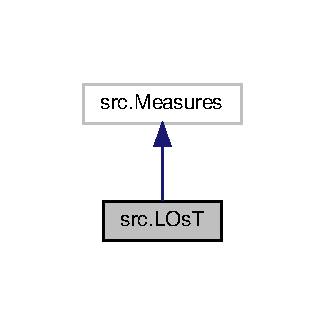
\includegraphics[width=156pt]{classsrc_1_1LOsT__inherit__graph}
\end{center}
\end{figure}


Collaboration diagram for src.\+L\+OsT\+:
\nopagebreak
\begin{figure}[H]
\begin{center}
\leavevmode
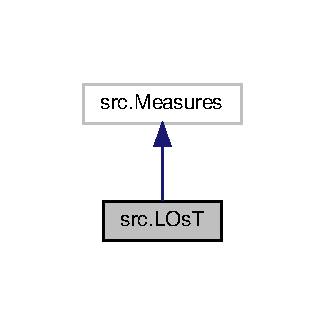
\includegraphics[width=156pt]{classsrc_1_1LOsT__coll__graph}
\end{center}
\end{figure}
\subsection*{Public Member Functions}
\begin{DoxyCompactItemize}
\item 
\mbox{\Hypertarget{classsrc_1_1LOsT_ae27763b81f31daeeabe518badd96635f}\label{classsrc_1_1LOsT_ae27763b81f31daeeabe518badd96635f}} 
{\bfseries L\+OsT} (String topic, int nblw, int nmrg, int nmts, int nexc)  throws Illegal\+Argument\+Exception
\item 
\mbox{\Hypertarget{classsrc_1_1LOsT_a02ef8179a6c3ffb078d78e10f83fdad3}\label{classsrc_1_1LOsT_a02ef8179a6c3ffb078d78e10f83fdad3}} 
String {\bfseries get\+Name} ()
\item 
\mbox{\Hypertarget{classsrc_1_1LOsT_a0ed196443c0d5b13a5acacfaf2a7c6fa}\label{classsrc_1_1LOsT_a0ed196443c0d5b13a5acacfaf2a7c6fa}} 
boolean {\bfseries equals} (Object o)
\item 
\mbox{\Hypertarget{classsrc_1_1LOsT_a2750f9ddf1a580cf01c0f40617cb707a}\label{classsrc_1_1LOsT_a2750f9ddf1a580cf01c0f40617cb707a}} 
double \mbox{[}$\,$\mbox{]} {\bfseries measures} ()
\item 
\mbox{\Hypertarget{classsrc_1_1LOsT_ac13be4bc4a4bc682ee2d2c244a0a7b87}\label{classsrc_1_1LOsT_ac13be4bc4a4bc682ee2d2c244a0a7b87}} 
double \mbox{[}$\,$\mbox{]} {\bfseries measures} (\hyperlink{enumsrc_1_1IndicatorT}{IndicatorT} ind)
\item 
\mbox{\Hypertarget{classsrc_1_1LOsT_aa2833e1ee68b2b20b2bdfbf92d032b18}\label{classsrc_1_1LOsT_aa2833e1ee68b2b20b2bdfbf92d032b18}} 
double \mbox{[}$\,$\mbox{]} {\bfseries measures} (\hyperlink{classsrc_1_1AttributeT}{AttributeT} att)
\end{DoxyCompactItemize}


The documentation for this class was generated from the following file\+:\begin{DoxyCompactItemize}
\item 
src/L\+Os\+T.\+java\end{DoxyCompactItemize}

\hypertarget{classsrc_1_1Norm}{}\section{src.\+Norm Class Reference}
\label{classsrc_1_1Norm}\index{src.\+Norm@{src.\+Norm}}
\subsection*{Static Public Member Functions}
\begin{DoxyCompactItemize}
\item 
\mbox{\Hypertarget{classsrc_1_1Norm_a75c929662a93db935c2b345ddccc9089}\label{classsrc_1_1Norm_a75c929662a93db935c2b345ddccc9089}} 
static void {\bfseries set\+Norms} (boolean n\+L\+Os, boolean n\+Ind, boolean n\+Att)
\item 
\mbox{\Hypertarget{classsrc_1_1Norm_a2e83c2e98568c8f6b7a63f881459bb2d}\label{classsrc_1_1Norm_a2e83c2e98568c8f6b7a63f881459bb2d}} 
static boolean {\bfseries get\+N\+L\+Os} ()
\item 
\mbox{\Hypertarget{classsrc_1_1Norm_a73dbfff5b03ad76ba811289ec321fff0}\label{classsrc_1_1Norm_a73dbfff5b03ad76ba811289ec321fff0}} 
static boolean {\bfseries get\+N\+Ind} ()
\item 
\mbox{\Hypertarget{classsrc_1_1Norm_a2838a0539243f3a9b40eef2cee7ebc5d}\label{classsrc_1_1Norm_a2838a0539243f3a9b40eef2cee7ebc5d}} 
static boolean {\bfseries get\+N\+Att} ()
\item 
\mbox{\Hypertarget{classsrc_1_1Norm_a0f504bea0d074ccf7ee218f04c7b6d9b}\label{classsrc_1_1Norm_a0f504bea0d074ccf7ee218f04c7b6d9b}} 
static void {\bfseries set\+N\+L\+Os} (boolean n\+L\+Os)
\item 
\mbox{\Hypertarget{classsrc_1_1Norm_a07feefb8d8498a5e7e5264caffca6f6e}\label{classsrc_1_1Norm_a07feefb8d8498a5e7e5264caffca6f6e}} 
static void {\bfseries set\+N\+Ind} (boolean n\+Ind)
\item 
\mbox{\Hypertarget{classsrc_1_1Norm_afe39f23f6fb7588bd4305f0f10c5e837}\label{classsrc_1_1Norm_afe39f23f6fb7588bd4305f0f10c5e837}} 
static void {\bfseries set\+N\+Att} (boolean n\+Att)
\end{DoxyCompactItemize}


The documentation for this class was generated from the following file\+:\begin{DoxyCompactItemize}
\item 
src/Norm.\+java\end{DoxyCompactItemize}

\hypertarget{classsrc_1_1ProgramT}{}\section{src.\+ProgramT Class Reference}
\label{classsrc_1_1ProgramT}\index{src.\+ProgramT@{src.\+ProgramT}}


Inheritance diagram for src.\+ProgramT\+:
\nopagebreak
\begin{figure}[H]
\begin{center}
\leavevmode
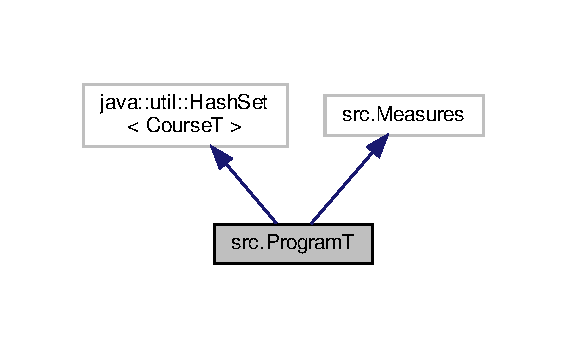
\includegraphics[width=272pt]{classsrc_1_1ProgramT__inherit__graph}
\end{center}
\end{figure}


Collaboration diagram for src.\+ProgramT\+:
\nopagebreak
\begin{figure}[H]
\begin{center}
\leavevmode
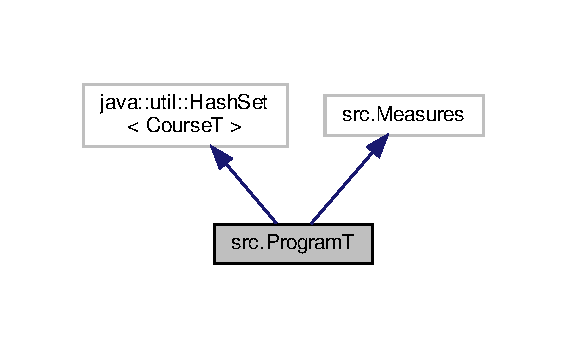
\includegraphics[width=272pt]{classsrc_1_1ProgramT__coll__graph}
\end{center}
\end{figure}
\subsection*{Public Member Functions}
\begin{DoxyCompactItemize}
\item 
\mbox{\Hypertarget{classsrc_1_1ProgramT_af9a7accf225be434e813dcc2792ca68a}\label{classsrc_1_1ProgramT_af9a7accf225be434e813dcc2792ca68a}} 
double \mbox{[}$\,$\mbox{]} {\bfseries measures} ()
\item 
\mbox{\Hypertarget{classsrc_1_1ProgramT_a2b00d3ad913d8301d97a47be686288bb}\label{classsrc_1_1ProgramT_a2b00d3ad913d8301d97a47be686288bb}} 
double \mbox{[}$\,$\mbox{]} {\bfseries measures} (\hyperlink{enumsrc_1_1IndicatorT}{IndicatorT} ind)
\item 
\mbox{\Hypertarget{classsrc_1_1ProgramT_a8585d325828de39c9d4d0ae70e3bc374}\label{classsrc_1_1ProgramT_a8585d325828de39c9d4d0ae70e3bc374}} 
double \mbox{[}$\,$\mbox{]} {\bfseries measures} (\hyperlink{classsrc_1_1AttributeT}{AttributeT} att)
\end{DoxyCompactItemize}


The documentation for this class was generated from the following file\+:\begin{DoxyCompactItemize}
\item 
src/Program\+T.\+java\end{DoxyCompactItemize}

\hypertarget{classsrc_1_1Services}{}\section{src.\+Services Class Reference}
\label{classsrc_1_1Services}\index{src.\+Services@{src.\+Services}}
\subsection*{Static Public Member Functions}
\begin{DoxyCompactItemize}
\item 
\mbox{\Hypertarget{classsrc_1_1Services_afb0da91ae8e15b6cdfbab39fcbf0fa9d}\label{classsrc_1_1Services_afb0da91ae8e15b6cdfbab39fcbf0fa9d}} 
static double \mbox{[}$\,$\mbox{]} {\bfseries normal} (double\mbox{[}$\,$\mbox{]} v)
\end{DoxyCompactItemize}


The documentation for this class was generated from the following file\+:\begin{DoxyCompactItemize}
\item 
src/Services.\+java\end{DoxyCompactItemize}

\chapter{File Documentation}
\hypertarget{CourseT_8java}{}\section{src/\+CourseT.java File Reference}
\label{CourseT_8java}\index{src/\+Course\+T.\+java@{src/\+Course\+T.\+java}}


Contains the Abstract Data Type for creating and operating with CourseT objects.  


\subsection*{Classes}
\begin{DoxyCompactItemize}
\item 
class \hyperlink{classsrc_1_1CourseT}{src.\+CourseT}
\begin{DoxyCompactList}\small\item\em Class for initializing and operating on \hyperlink{classsrc_1_1CourseT}{CourseT} objects. \end{DoxyCompactList}\end{DoxyCompactItemize}
\subsection*{Packages}
\begin{DoxyCompactItemize}
\item 
package \hyperlink{namespacesrc}{src}
\end{DoxyCompactItemize}


\subsection{Detailed Description}
Contains the Abstract Data Type for creating and operating with CourseT objects. 

\begin{DoxyAuthor}{Author}
Mohammad Omar Zahir -\/ zahirm1 
\end{DoxyAuthor}
\begin{DoxyDate}{Date}
March 29, 2021 
\end{DoxyDate}

%--- End generated contents ---

% Index
\backmatter
\newpage
\phantomsection
\clearemptydoublepage
\addcontentsline{toc}{chapter}{Index}
\printindex

\end{document}
